% ---------------------------------------------------------------- 24 Nov 2026: cavern-rock x mu vertices with the pair lines, and vertex z (4-station + TD, preliminary)
\begin{btframe}{7 · Back-up · cavern-rock × μ vertices}{Cavern-rock × μ vertices in the vessel (4 stations + TD, preliminary)}
\centering
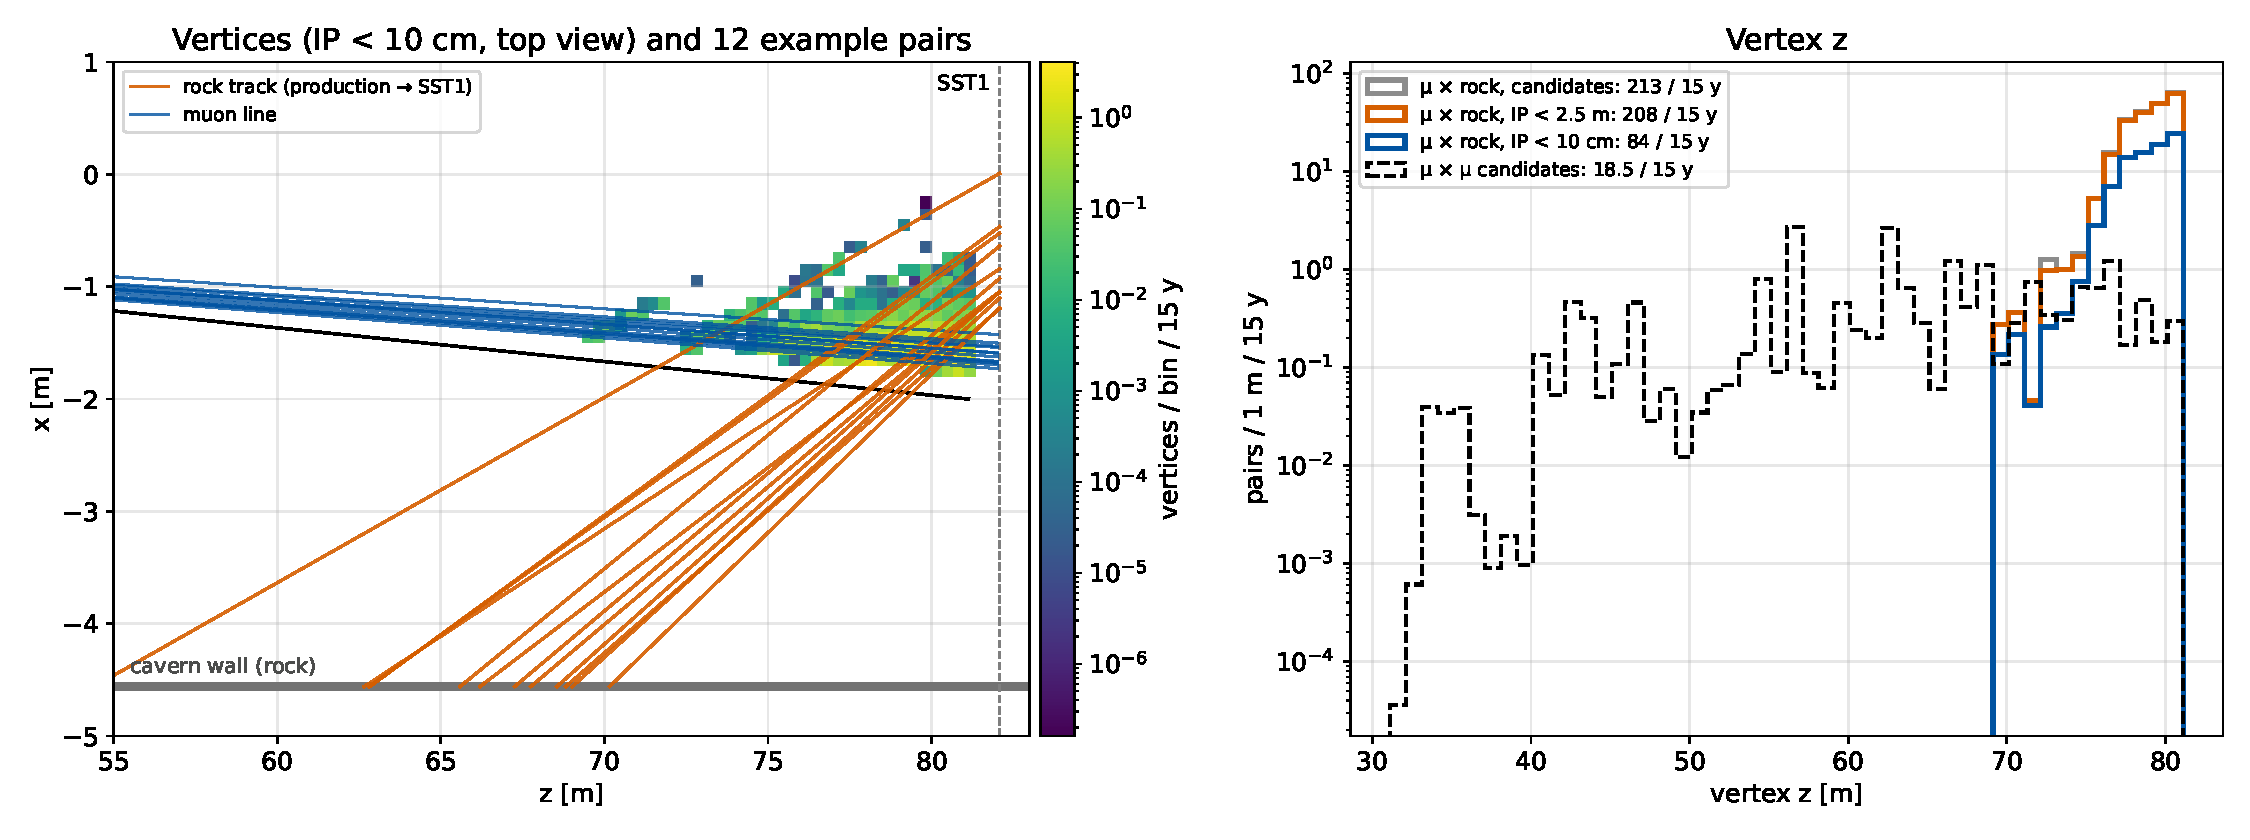
\includegraphics[width=0.96\linewidth,height=170pt,keepaspectratio]{figs/s48_rock_mu_vertices.pdf}\par
\vspace{4pt}
\raggedright
\begin{itemize}\footnotesize
  \item Left: vertices of the pairs with measured IP < 10 cm (top view, per 15 y) and 12 example pairs: rock tracks (orange) from the −x cavern wall cross the muon lines (blue) just inside the −x vessel wall
  \item Right: vertex z at each cut, μ × μ for comparison: all μ × rock vertices in the last ~10 m of the vessel (median 79.2 m), μ × μ spread over the whole vessel
\end{itemize}
\end{btframe}
